%% aframe_software_arch.tex  –  High-level software architecture
%% Compile:  pdflatex aframe_software_arch.tex && pdfcrop aframe_software_arch.pdf
\documentclass{article}
\usepackage[margin=1cm, paperwidth=30cm, paperheight=18cm]{geometry}
\pagestyle{empty}
\usepackage{tikz}
\usetikzlibrary{positioning,arrows.meta,fit,backgrounds,calc}

\colorlet{srcfill} {gray!15}   \colorlet{srcbrd}  {gray!55}
\colorlet{mainfill}{blue!10}   \colorlet{mainbrd} {blue!55!black}
\colorlet{subfill} {orange!12} \colorlet{subbrd}  {orange!65!black}
\colorlet{qfill}   {teal!10}   \colorlet{qbrd}    {teal!55!black}
\colorlet{extfill} {purple!12} \colorlet{extbrd}  {purple!55!black}

\begin{document}
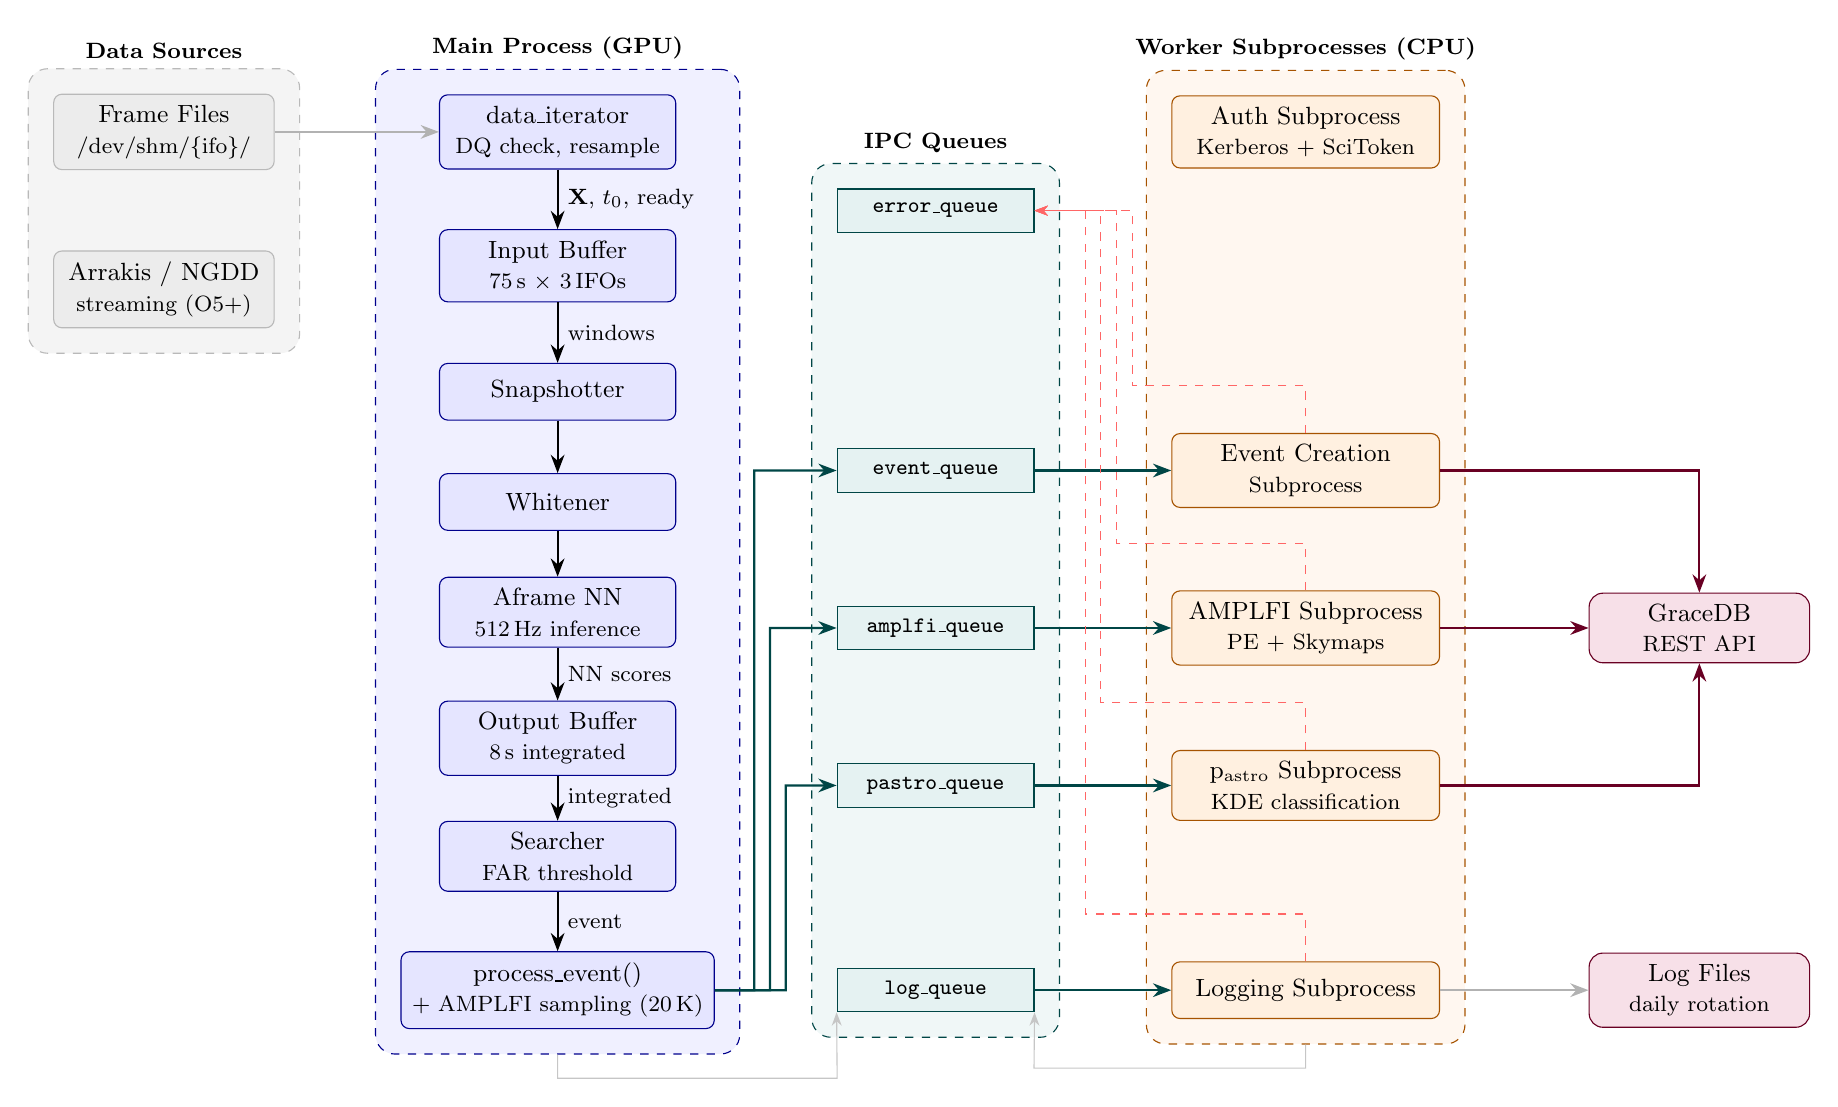
\begin{tikzpicture}[
  >=Stealth,
  every node/.style={font=\small, align=center},
  src/.style  ={draw=srcbrd,  fill=srcfill,  rounded corners=3pt,
                minimum width=2.8cm, minimum height=0.72cm, inner sep=4pt},
  main/.style ={draw=mainbrd, fill=mainfill, rounded corners=3pt,
                minimum width=3.0cm, minimum height=0.72cm, inner sep=4pt},
  sub/.style  ={draw=subbrd,  fill=subfill,  rounded corners=3pt,
                minimum width=3.4cm, minimum height=0.72cm, inner sep=4pt},
  qnode/.style={draw=qbrd, fill=qfill,
                minimum width=2.5cm, minimum height=0.55cm,
                inner sep=3pt, font=\footnotesize\ttfamily},
  ext/.style  ={draw=extbrd, fill=extfill, rounded corners=5pt,
                minimum width=2.8cm, minimum height=0.72cm, inner sep=4pt},
  arr/.style   ={->, thick},
  earr/.style  ={->, thick, gray!60},
  qarr/.style  ={->, thick, qbrd},
  garr/.style  ={->, thick, extbrd},
  grdarr/.style={->, thick, green!45!black},
  radr/.style  ={->, dashed, red!60},
  grp/.style   ={draw, dashed, rounded corners=7pt, inner sep=9pt},
]

%% ── Column 1: Data Sources (x = 0) ───────────────────────────────────────
\node[src] (shm)  at (0, 9.5) {Frame Files\\{\footnotesize /dev/shm/\{ifo\}/}};
\node[src] (ngdd) at (0, 7.5) {Arrakis / NGDD\\{\footnotesize streaming (O5+)}};

%% ── Column 2: Main Process (x = 5) ──────────────────────────────────────
\node[main] (datait) at (5, 9.5) {data\_iterator\\{\footnotesize DQ check, resample}};
\node[main] (inbuf)  at (5, 7.8) {Input Buffer\\{\footnotesize 75\,s $\times$ 3\,IFOs}};
\node[main] (snap)   at (5, 6.2) {Snapshotter};
\node[main] (white)  at (5, 4.8) {Whitener};
\node[main] (aframe) at (5, 3.4) {Aframe NN\\{\footnotesize 512\,Hz inference}};
\node[main] (outbuf) at (5, 1.8) {Output Buffer\\{\footnotesize 8\,s integrated}};
\node[main] (srch)   at (5, 0.3) {Searcher\\{\footnotesize FAR threshold}};
\node[main] (pevt)   at (5,-1.4) {process\_event()\\{\footnotesize + AMPLFI sampling (20\,K)}};

%% ── Column 3: IPC Queues (x = 9.8) ──────────────────────────────────────
\node[qnode] (errq) at (9.8, 8.5)  {error\_queue};
\node[qnode] (evtq) at (9.8, 5.2)  {event\_queue};
\node[qnode] (ampq) at (9.8, 3.2)  {amplfi\_queue};
\node[qnode] (pasq) at (9.8, 1.2)  {pastro\_queue};
\node[qnode] (logq) at (9.8,-1.4)  {log\_queue};

%% ── Column 4: Subprocesses (x = 14.5) ───────────────────────────────────
\node[sub] (authsp) at (14.5, 9.5) {Auth Subprocess\\{\footnotesize Kerberos + SciToken}};
\node[sub] (evtsp)  at (14.5, 5.2) {Event Creation\\{\footnotesize Subprocess}};
\node[sub] (ampsp)  at (14.5, 3.2) {AMPLFI Subprocess\\{\footnotesize PE + Skymaps}};
\node[sub] (passp)  at (14.5, 1.2) {p$_{\mathrm{astro}}$ Subprocess\\{\footnotesize KDE classification}};
\node[sub] (logsp)  at (14.5,-1.4) {Logging Subprocess};

%% ── Column 5: External Services (x = 19.5) ──────────────────────────────
\node[ext] (gdb)    at (19.5, 3.2) {GraceDB\\{\footnotesize REST API}};
\node[ext] (logfil) at (19.5,-1.4) {Log Files\\{\footnotesize daily rotation}};

%% ════════════════════════════════════════════════════════════
%% ARROWS
%% ════════════════════════════════════════════════════════════

%% Data sources → data_iterator
\draw[earr] (shm.east) -- ++(1.0,0) |- (datait.west);

%% Main process vertical flow
\draw[arr] (datait) -- node[right, font=\footnotesize]{$\mathbf{X}$, $t_0$, ready} (inbuf);
\draw[arr] (inbuf)  -- node[right, font=\footnotesize]{windows} (snap);
\draw[arr] (snap)   -- (white);
\draw[arr] (white)  -- (aframe);
\draw[arr] (aframe) -- node[right, font=\footnotesize]{NN scores} (outbuf);
\draw[arr] (outbuf) -- node[right, font=\footnotesize]{integrated} (srch);
\draw[arr] (srch)   -- node[right, font=\footnotesize]{event} (pevt);

%% process_event → queues (separate vertical segments to avoid overlap)
\draw[qarr] (pevt.east) -- ++(0.5,0) -- ++(0,6.6) -- (evtq.west);
\draw[qarr] (pevt.east) -- ++(0.7,0) -- ++(0,4.6) -- (ampq.west);
\draw[qarr] (pevt.east) -- ++(0.9,0) -- ++(0,2.6) -- (pasq.west);


%% Queues → subprocesses
\draw[qarr] (evtq) -- (evtsp);
\draw[qarr] (ampq) -- (ampsp);
\draw[qarr] (pasq) -- (passp);
\draw[qarr] (logq) -- (logsp);


%% Error queue: subprocesses send errors at different horizontal levels
\draw[radr] (evtsp.north) -- ++(0,0.6) -- ++(-2.2,0) |- (errq.east);
\draw[radr] (ampsp.north) -- ++(0,0.6) -- ++(-2.4,0) |- (errq.east);
\draw[radr] (passp.north) -- ++(0,0.6) -- ++(-2.6,0) |- (errq.east);
\draw[radr] (logsp.north) -- ++(0,0.6) -- ++(-2.8,0) |- (errq.east);
% \draw[radr, <-]
%   (errq.west) -- ++(-1.55,0) -- ++(0,-8.2) -- (srch.east)
%   node[pos=0.15, above, font=\footnotesize, red!60]{monitor};

%% Subprocesses → external services
\draw[garr] (evtsp.east) -- ++(0.5,0) -| (gdb.north);
\draw[garr] (ampsp.east) -- (gdb.west);
\draw[garr] (passp.east) -- ++(0.5,0) -| (gdb.south);
\draw[earr] (logsp.east) -- (logfil.west);

%% ════════════════════════════════════════════════════════════
%% BACKGROUND GROUP BOXES
%% ════════════════════════════════════════════════════════════
\begin{pgfonlayer}{background}
  \node[grp, draw=srcbrd,  fill=srcfill!60,
        label={[font=\footnotesize\bfseries]above:Data Sources}]
    [fit=(shm)(ngdd)] {};
  \node[grp, draw=mainbrd, fill=mainfill!60,
        label={[font=\footnotesize\bfseries]above:Main Process (GPU)}]
    (maingrp) [fit=(datait)(pevt)] {};
  \node[grp, draw=qbrd,    fill=qfill!60,
        label={[font=\footnotesize\bfseries]above:IPC Queues}]
    [fit=(errq)(logq)] {};
  \node[grp, draw=subbrd,  fill=subfill!50,
        label={[font=\footnotesize\bfseries]above:Worker Subprocesses (CPU)}]
    (subgrp) [fit=(authsp)(evtsp)(ampsp)(passp)(logsp)] {};
\end{pgfonlayer}

%% Logging: both group bounding boxes → log_queue, routed below content
\draw[qarr, thin, gray!45]
  (maingrp.south) -- ++(0,-0.3) -- ++(3.55,0) -- (logq.south west);
\draw[qarr, thin, gray!45]
  (subgrp.south) -- ++(0,-0.3) -- ++(-3.45,0) -- (logq.south east);

\end{tikzpicture}
\end{document}
